\documentclass{standalone}
\usepackage{tikz}
\usetikzlibrary{patterns, positioning}


\begin{document}
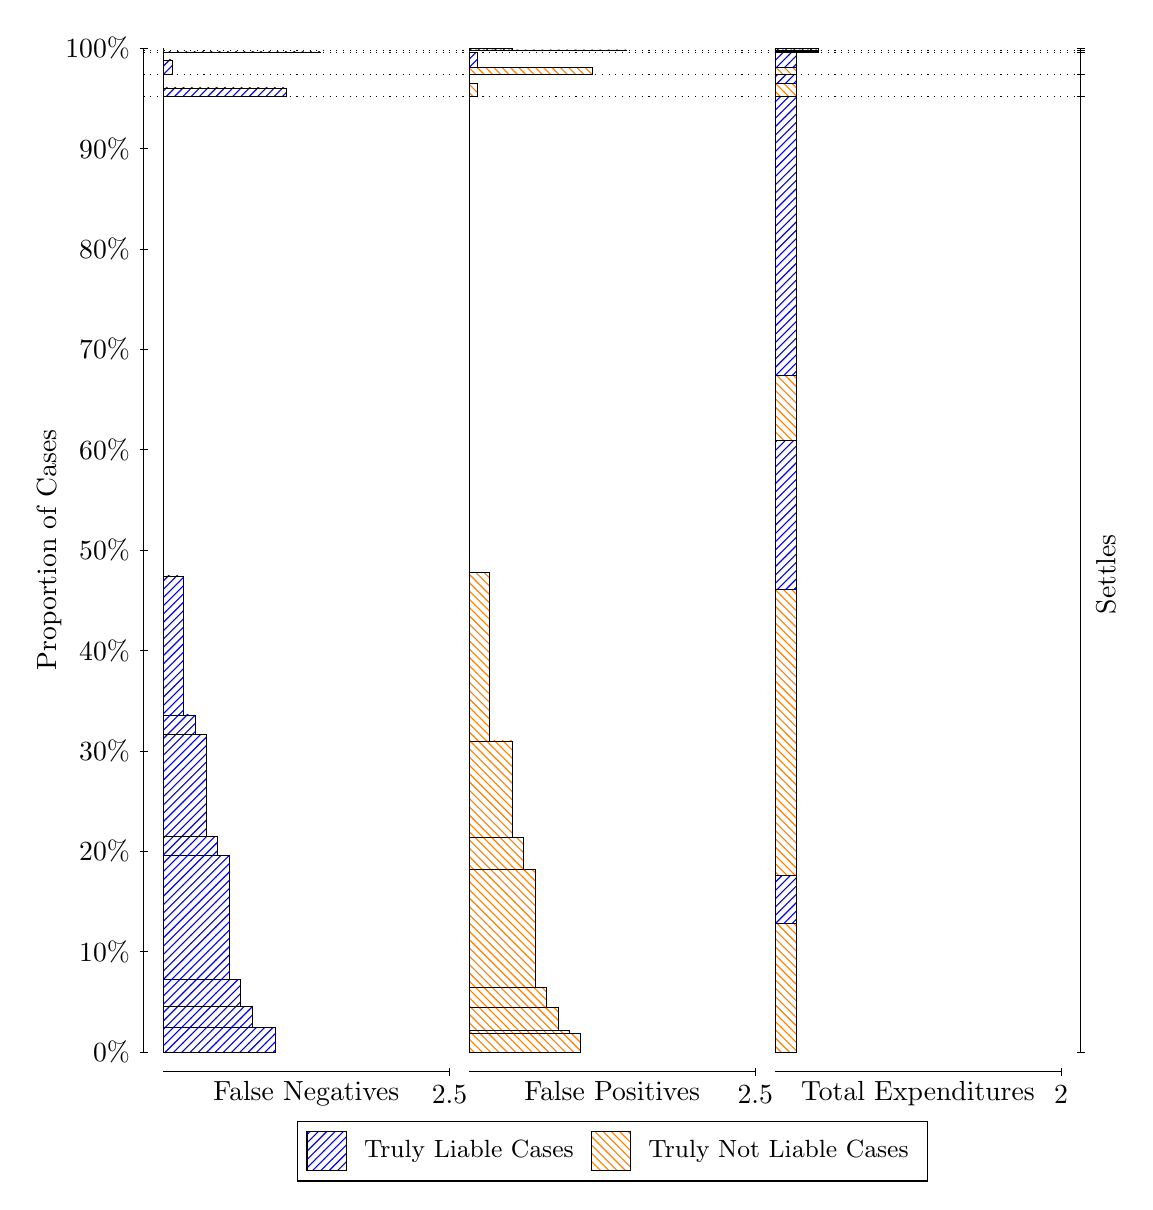
\begin{tikzpicture}
\draw[black, very thin] (1.5,1.75) -- (1.5,14.5);
\node[rotate=90, text=black, anchor=center] at (0.3, 8.125) {Proportion of Cases};
\draw[black, very thin] (1.45,1.75) -- (1.55,1.75);
\node[text=black, anchor=east] at (1.45, 1.75) {0\%};
\draw[black, very thin] (1.45,3.025) -- (1.55,3.025);
\node[text=black, anchor=east] at (1.45, 3.025) {10\%};
\draw[black, very thin] (1.45,4.3) -- (1.55,4.3);
\node[text=black, anchor=east] at (1.45, 4.3) {20\%};
\draw[black, very thin] (1.45,5.575) -- (1.55,5.575);
\node[text=black, anchor=east] at (1.45, 5.575) {30\%};
\draw[black, very thin] (1.45,6.85) -- (1.55,6.85);
\node[text=black, anchor=east] at (1.45, 6.85) {40\%};
\draw[black, very thin] (1.45,8.125) -- (1.55,8.125);
\node[text=black, anchor=east] at (1.45, 8.125) {50\%};
\draw[black, very thin] (1.45,9.4) -- (1.55,9.4);
\node[text=black, anchor=east] at (1.45, 9.4) {60\%};
\draw[black, very thin] (1.45,10.675) -- (1.55,10.675);
\node[text=black, anchor=east] at (1.45, 10.675) {70\%};
\draw[black, very thin] (1.45,11.95) -- (1.55,11.95);
\node[text=black, anchor=east] at (1.45, 11.95) {80\%};
\draw[black, very thin] (1.45,13.225) -- (1.55,13.225);
\node[text=black, anchor=east] at (1.45, 13.225) {90\%};
\draw[black, very thin] (1.45,14.5) -- (1.55,14.5);
\node[text=black, anchor=east] at (1.45, 14.5) {100\%};

\draw[black, very thin] (13.4,1.75) -- (13.4,14.5);
\draw[black, very thin] (13.35,1.75) -- (13.45,1.75);
\node[anchor=west] at (13.35, 1.75) {};
\draw[black, very thin] (13.35,13.884) -- (13.45,13.884);
\node[anchor=west] at (13.35, 13.884) {};
\draw[black, very thin] (13.35,14.163) -- (13.45,14.163);
\node[anchor=west] at (13.35, 14.163) {};
\draw[black, very thin] (13.35,14.44) -- (13.45,14.44);
\node[anchor=west] at (13.35, 14.44) {};
\draw[black, very thin] (13.35,14.467) -- (13.45,14.467);
\node[anchor=west] at (13.35, 14.467) {};
\draw[black, very thin] (13.35,14.5) -- (13.45,14.5);
\node[anchor=west] at (13.35, 14.5) {};

\draw[black, very thin, pattern color=blue, pattern=north east lines] (1.75,1.75) rectangle (3.167,2.066);
\draw[black, very thin, pattern color=blue, pattern=north east lines] (1.75,2.066) rectangle (2.8763,2.331);
\draw[black, very thin, pattern color=blue, pattern=north east lines] (1.75,2.331) rectangle (2.731,2.6755);
\draw[black, very thin, pattern color=blue, pattern=north east lines] (1.75,2.6755) rectangle (2.5857,4.2515);
\draw[black, very thin, pattern color=blue, pattern=north east lines] (1.75,4.2515) rectangle (2.4403,4.4898);
\draw[black, very thin, pattern color=blue, pattern=north east lines] (1.75,4.4898) rectangle (2.295,5.7786);
\draw[black, very thin, pattern color=blue, pattern=north east lines] (1.75,5.7786) rectangle (2.1497,6.0302);
\draw[black, very thin, pattern color=blue, pattern=north east lines] (1.75,6.0302) rectangle (2.0043,7.7974);
\draw[black, very thin, pattern color=orange, pattern=north west lines] (1.75,7.7974) rectangle (1.75,13.884);
\draw[black, very thin, pattern color=blue, pattern=north east lines] (1.75,13.884) rectangle (3.3123,13.993);
\draw[black, very thin, pattern color=orange, pattern=north west lines] (1.75,13.993) rectangle (1.75,14.163);
\draw[black, very thin, pattern color=blue, pattern=north east lines] (1.75,14.163) rectangle (1.859,14.349);
\draw[black, very thin, pattern color=orange, pattern=north west lines] (1.75,14.349) rectangle (1.75,14.44);
\draw[black, very thin, pattern color=blue, pattern=north east lines] (1.75,14.44) rectangle (3.7483,14.45);
\draw[black, very thin, pattern color=orange, pattern=north west lines] (1.75,14.45) rectangle (1.75,14.467);
\draw[black, very thin, pattern color=orange, pattern=north west lines] (1.75,14.467) rectangle (1.75,14.477);
\draw[black, very thin, pattern color=blue, pattern=north east lines] (1.75,14.477) rectangle (1.75,14.5);
\draw[black, very thin, pattern color=orange, pattern=north west lines] (5.6333,1.75) rectangle (7.0503,1.9851);
\draw[black, very thin, pattern color=orange, pattern=north west lines] (5.6333,1.9851) rectangle (6.905,2.0249);
\draw[black, very thin, pattern color=orange, pattern=north west lines] (5.6333,2.0249) rectangle (6.7597,2.3205);
\draw[black, very thin, pattern color=orange, pattern=north west lines] (5.6333,2.3205) rectangle (6.6143,2.5664);
\draw[black, very thin, pattern color=orange, pattern=north west lines] (5.6333,2.5664) rectangle (6.469,4.0663);
\draw[black, very thin, pattern color=orange, pattern=north west lines] (5.6333,4.0663) rectangle (6.3237,4.4793);
\draw[black, very thin, pattern color=orange, pattern=north west lines] (5.6333,4.4793) rectangle (6.1783,5.7005);
\draw[black, very thin, pattern color=orange, pattern=north west lines] (5.6333,5.7005) rectangle (5.8877,7.8366);
\draw[black, very thin, pattern color=blue, pattern=north east lines] (5.6333,7.8366) rectangle (5.6333,13.884);
\draw[black, very thin, pattern color=orange, pattern=north west lines] (5.6333,13.884) rectangle (5.7423,14.054);
\draw[black, very thin, pattern color=blue, pattern=north east lines] (5.6333,14.054) rectangle (5.6333,14.163);
\draw[black, very thin, pattern color=orange, pattern=north west lines] (5.6333,14.163) rectangle (7.1957,14.254);
\draw[black, very thin, pattern color=blue, pattern=north east lines] (5.6333,14.254) rectangle (5.7423,14.44);
\draw[black, very thin, pattern color=orange, pattern=north west lines] (5.6333,14.44) rectangle (5.6333,14.457);
\draw[black, very thin, pattern color=blue, pattern=north east lines] (5.6333,14.457) rectangle (5.6333,14.467);
\draw[black, very thin, pattern color=orange, pattern=north west lines] (5.6333,14.467) rectangle (7.6317,14.477);
\draw[black, very thin, pattern color=blue, pattern=north east lines] (5.6333,14.477) rectangle (6.1783,14.5);
\draw[black, very thin, pattern color=orange, pattern=north west lines] (9.5167,1.75) rectangle (9.7892,3.3842);
\draw[black, very thin, pattern color=blue, pattern=north east lines] (9.5167,3.3842) rectangle (9.7892,3.9936);
\draw[black, very thin, pattern color=orange, pattern=north west lines] (9.5167,3.9936) rectangle (9.7892,7.6296);
\draw[black, very thin, pattern color=blue, pattern=north east lines] (9.5167,7.6296) rectangle (9.7892,9.5217);
\draw[black, very thin, pattern color=orange, pattern=north west lines] (9.5167,9.5217) rectangle (9.7892,10.338);
\draw[black, very thin, pattern color=blue, pattern=north east lines] (9.5167,10.338) rectangle (9.7892,13.884);
\draw[black, very thin, pattern color=orange, pattern=north west lines] (9.5167,13.884) rectangle (9.7892,14.054);
\draw[black, very thin, pattern color=blue, pattern=north east lines] (9.5167,14.054) rectangle (9.7892,14.163);
\draw[black, very thin, pattern color=orange, pattern=north west lines] (9.5167,14.163) rectangle (9.7892,14.254);
\draw[black, very thin, pattern color=blue, pattern=north east lines] (9.5167,14.254) rectangle (9.7892,14.44);
\draw[black, very thin, pattern color=orange, pattern=north west lines] (9.5167,14.44) rectangle (10.062,14.457);
\draw[black, very thin, pattern color=blue, pattern=north east lines] (9.5167,14.457) rectangle (10.062,14.467);
\draw[black, very thin, pattern color=orange, pattern=north west lines] (9.5167,14.467) rectangle (10.062,14.477);
\draw[black, very thin, pattern color=blue, pattern=north east lines] (9.5167,14.477) rectangle (10.062,14.5);
\draw[black, dotted] (1.5,13.884) -- (13.4,13.884);
\draw[black, dotted] (1.5,14.163) -- (13.4,14.163);
\draw[black, dotted] (1.5,14.44) -- (13.4,14.44);
\draw[black, dotted] (1.5,14.467) -- (13.4,14.467);
\draw[black, very thin] (1.75,1.5) -- (5.3833,1.5);
\node[text=black, anchor=north] at (3.5667, 1.5) {False Negatives};
\draw[black, very thin] (5.3833,1.45) -- (5.3833,1.55);
\node[text=black, anchor=north] at (5.3833, 1.45) {2.5};

\draw[black, very thin] (5.6333,1.5) -- (9.2667,1.5);
\node[text=black, anchor=north] at (7.45, 1.5) {False Positives};
\draw[black, very thin] (9.2667,1.45) -- (9.2667,1.55);
\node[text=black, anchor=north] at (9.2667, 1.45) {2.5};

\draw[black, very thin] (9.5167,1.5) -- (13.15,1.5);
\node[text=black, anchor=north] at (11.333, 1.5) {Total Expenditures};
\draw[black, very thin] (13.15,1.45) -- (13.15,1.55);
\node[text=black, anchor=north] at (13.15, 1.45) {2};

\node[text=black, centered, rotate=90] at (13.72, 7.817) {Settles};





\draw (7.449999999999999,1.5) node[draw=none] (baseCoordinate) {};
\begin{scope}[align=center]
        \matrix[scale=0.5, draw=black, below=0.5cm of baseCoordinate, nodes={draw}, column sep=0.1cm]{
            \node[rectangle, draw, minimum width=0.5cm, minimum height=0.5cm, pattern color=blue, pattern=north east lines] {}; &
            \node[draw=none, font=\small, text=black] (B) {Truly Liable Cases}; &
            \node[rectangle, draw, minimum width=0.5cm, minimum height=0.5cm, pattern color=orange, pattern=north west lines] {}; &
            \node[draw=none, font=\small, text=black] (B) {Truly Not Liable Cases}; \\
            };
\end{scope}

\end{tikzpicture}
\end{document}